\section{کارهای پیشین}\label{review}
در تحقیقات پیشین، از روش‌های متعددی برای توصیف ویدئو‌ها استفاده شده است. به طور کلی می‌توان این‌ روش‌ها را به دو دسته‌ی روش‌های سنتی و روش‌های مبتنی بر شبکه‌های ژرف تقسیم کرد. عموم روش‌های سنتی بدین صورت عمل می‌کنند که ابتدا با استفاده از مجموعه‌ای از ویژگی‌های دست‌ساز، با استفاده از الگوریتم‌های شناسایی اشیاء یا کنش‌ها، یک باز‌نمایش از اشیاء و کنش‌های موجود در تصویر به دست می‌آورند و سپس تلاش می‌کنند دانش به‌دست آمده از ویژگی‌های تصویری را به نحوی با دانش به دست آمده از روش‌های پردازش زبان طبیعی مخلوط کنند و به مدلی دست یابند که عملکرد مناسبی در ایجاد جملات به زبان طبیعی داشته باشد. برای مثال در \cite{Krishnamoorthy2013}، نویسندگان یک روش سه مرحله‌ای برای توصیف ویدئو‌ها ارائه می‌دهند. در گام اول این روش، با استفاده از الگوریتم‌های بازشناسی تصویر، اشیاء و کنش‌های موجود در ویدئو استخراج می‌شوند. در ادامه و درگام دوم، با استفاده از تخمین بیشینه‌ی درست نمایی 
\LTRfootnote{Maximum Likelihood Estimation}
از دنیای واقعی، که با کاوش‌کردن سه‌بخشی‌های فعل، فاعل و مفعول از متون موجود در اینترنت به دست آمده است، یافته‌های گام اول را با دانش موجود از کاوش متون، مخلوط می‌کنند تا بهترین سه‌تایی را به دست آورند. در ادامه و در گام نهایی، با استفاده از مجموعه‌ای از جملات قالب (از قبل تعیین شده)، جملات نهایی ایجاد شده و بر اساس روان‌ و منطقی بودن رده‌بندی می‌شوند و بهترین جمله انتخاب می‌شود.

باید دقت داشت که با توجه به ابعاد بسیار بزرگ فضای ویودئو، ابتدا لازم است که این فضا خود به فضایی کوچک‌تر نگاشت شود. به همین دلیل عموم‌ روش‌های پیشین ارائه شده، ابتدا از فریم‌های مختلف ویدئو نمونه‌برداری می‌کنند و سپس با استفاده از شبکه‌‌های ژرف پیچشی، سعی در شناسایی یک فضای میانی کوچک‌تر برای فریم‌ها می‌کنند (استخراج ویژگی). در نهایت نیز با توجه به هدف مسئله از یک دسته‌بند (شبکه‌ی کاملا متصل \LTRfootnote{Fully‌ Connected Network} یا دسته‌بند‌های سنتی مانند ماشین‌های بردار پشتیبان  \LTRfootnote{Support Vector ‌Machine}یا درخت‌تصمیم \LTRfootnote{Decision‌ Tree}) و یا یک شبکه‌‌ی بازگردنده \LTRfootnote{Recurrent Neural‌‌‌ Networks} استفاده می‌کنند.

در این بخش، با توجه به فراگیری این چارچوب به مرور دقیق‌تر روش‌های پیشنهاد شده‌ی پیشین برای حل این مسئله می‌پردازیم. 
  
\subsection{ایجاد توصیف با استفاده از دانش متن‌کاوی شده}\label{text-mined-knowledge}
در این روش، نویسندگان پژوهش
\cite{Krishnamoorthy2013} 
 مدلی را ارائه می‌دهند که با در نظر گرفتن مخلوطی از دانش به دست آمده از حوزه‌ی پردازش‌زبان‌طبیعی و روش‌های بینایی‌رایانه‌ای، به ایجاد جملات توصیف‌کننده برای ویدئو‌ها می‌پردازد. این مدل از دو مرحله‌ی اصلی تشکیل شده است. در مرحله‌ی اول، محتمل‌ترین فعل، فاعل و مفعول، با توجه به محتوا تصویر (روش‌‌های بینایی‌رایانه‌ای) و احتمال کنار‌هم قرارگیری این سه کلمه (روش‌های پردازش‌ زبان‌ طبیعی) استخراج می‌شوند. به این مرحله، مرحله‌ی برنامه‌ریزی محتوا 
\LTRfootnote{Content Planning Stage}
  نیز گفته می‌شود. سپس در مرحله‌ی دوم، با توجه به سه‌ کلمه‌ی به دست آمده در مرحله‌ی قبل و با استفاده از یک روش ساده‌ی مبتی بر قالب، جملات توصیف‌گر ورودی ایجاد می‌شوند. این جملات در نهایت با استفاده از یک مدل زبانی‌ احتمالاتی که روی داده‌های متنی موجود در اینترنت آموزش داده‌ شده است، رده‌بندی می‌شوند تا بهترین جمله‌ی توصیف‌کننده‌ی یک ویدئو انتخاب شود. به این مرحله‌، مرحله‌ی تحقق سطح 
\LTRfootnote{Surface Realization}
   گفته‌ می‌شود. در تصویر 
\ref{text-mined-knowledge-model-1} 
   شمایی از این مدل قابل مشاهده‌ است.
\begin{figure}[h]
	\centering
	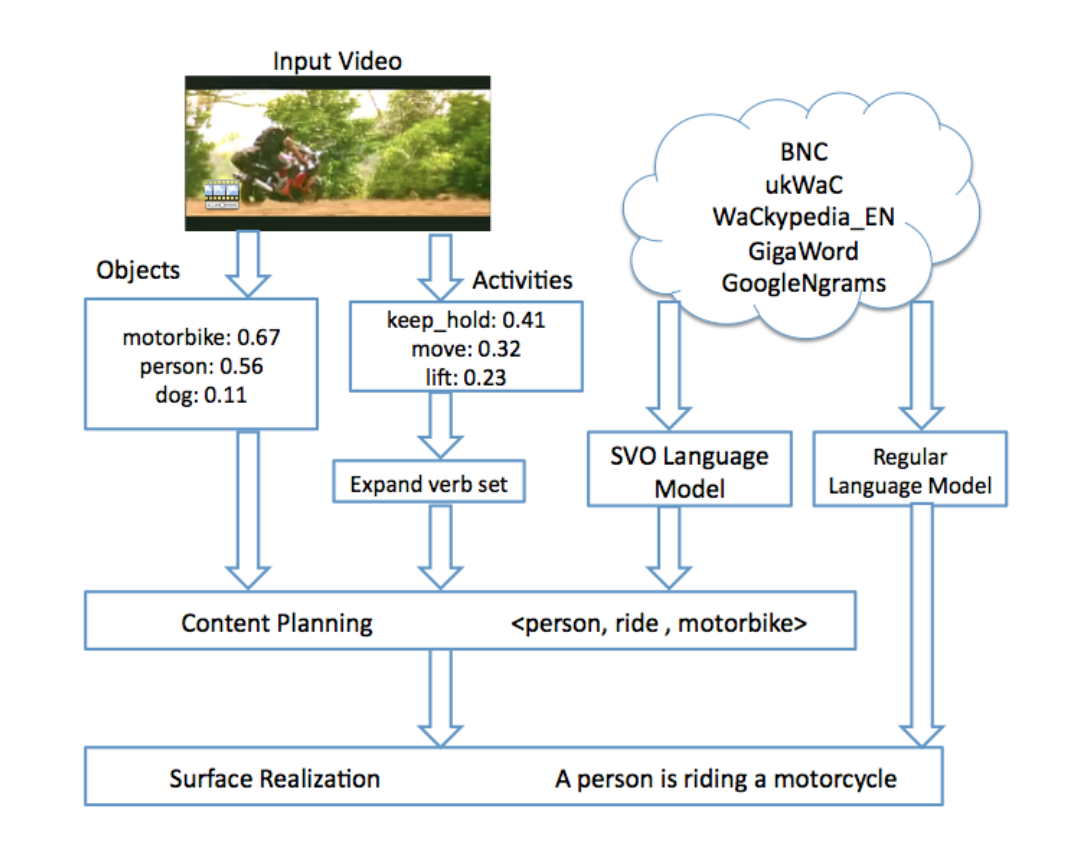
\includegraphics[width=120mm]{images/Text-mined-knowledge-model.png}
	\caption{برنامه‌ریزی محتوا و تحقق سطح \label{text-mined-knowledge-model-1}\cite{Krishnamoorthy2013}}
\end{figure}
نویسندگان در این پژوهش، ابتدا اشیاء و کنش‌های موجود در ویدئو را با استفاده از مدل‌های بازشناسی تصویر به دست می‌آورند. با توجه به اینکه این اطلاعات عموماً دارای نوفه
\LTRfootnote{Noise}
 و خطای قابل توجهی هستند، گام بعدی توسط نویسندگان پیشنهاد شده است. در این گام، با در نظر گرفتن احتمال قرار‌گرفتن اشیاء و کنش‌های تشخیص داده‌شده در مرحله‌ی قبل، در متون موجود در منابع مختلف، محتمل‌ترین فعل،‌ فاعل و مفعول استخراج می‌شوند. در نهایت نیز پیش‌بینی‌ها با قرار گرفتن در قالب‌های متفاوت نمره‌دهی و رتبه‌بندی می‌شوند تا بهترین جمله‌ی توصیف‌کننده انتخاب شود.

در این روش
\ref{text-mined-knowledge-model-1}
 برای بازشناسی اشیاء از روش ارائه شده در 
\cite{felzenszwalb2008discriminatively}
 استفاده می‌شود. همچنین برای شناسایی کنش‌های موجود در ویدئو از مدل ارائه شده توسط 
\cite{laptev2008learning}
 استفاده می‌شود. در این روش  ویژگی‌ها، بافت‌نگار‌ بردار‌های گرادیان 
\LTRfootnote{Histogram Of Gradients}
  و شارش‌نوری 
\LTRfootnote{Histogram Of Optical Flow} 
  هستند که روی نقاط پراهمیت مکانی-زمانی 
\LTRfootnote{Spatio-temporal interest points}
   محاسبه می‌شوند. در گام بعدی با اجرای خوشه‌بندی روی این ویژگی‌ها، یک نمایش کیسه‌کلمات 
\LTRfootnote{Bag of Words}
   برای هر خوشه از ویژگی‌ها به دست می‌آید که با تجمیع این نمایش برای تمامی فریم‌ها، بازنمایش نهایی ویدئو به صورت بافت‌نگاری از نمایش‌های  کیسه کلمات به دست می‌آید. در نهایت با آموزش دادن یک مدل دسته‌بند (مانند ماشین‌های بردار پشتیبان)، عمل رخ‌داده‌شده در ویدئو شناسایی می‌شود. در مرحله‌ی برنامه‌ریزی محتوا، اطلاعات مرتبط با تصویر با استفاده از رابطه‌ی زیر، با اطلاعات به دست آمده از متون، مخلوط می‌شوند تا بهترین سه‌تایی‌های فعل، فاعل و مفعول به دست آیند.
 \begin{equation} \label{text-mined-knowledge-model-1-visScore}
visScore = p(S|vid)*p(V_{orig}|vid)*sim(V_{sim}, V_{orig})*p(O|vid)
 \end{equation} 
 \begin{equation} \label{text-mined-knowledge-model-1-score}
   score = w_1‌*‌visScore‌+ w_2 *‌nlpScore
 \end{equation} 
در رابطه‌ی
 \ref{text-mined-knowledge-model-1-visScore}
 ، منظور از 
$V_{sim}$
مجموعه‌ای از افعال اضافی و مشابه‌ با افعال شناسایی شده در مرحله‌ی قبل است که با توجه به یک دسته‌بندی قبلی توسط نویسندگان، در کنار هر فعل در نظر گرفته می‌شود. (به عنوان مثال برای فعل حرکت‌کردن، افعال راه‌رفتن، دویدن و رد کردن نیز در نظر گرفته می‌شود). در مرحله‌ی بعد، سه‌ کلمه‌ی انتخاب شده در قالب‌هایی آماده برای جملات قرار می‌گیرند، جملات ساخته‌شده توسط مدل زبانی 
\cite{pauls2011faster}
امتیاز دهی می‌شوند و در نهایت بهترین جمله، جمله‌ با بالاترین امتیاز،‌ انتخاب می‌شود. نمونه‌ای از قالب‌های استفاده شده به صورت مقابل است:
\LR{
"A/The, Subject, Verb‌, Preposition (optional), A/The, Object"
}

در مطالعه‌ی 
\cite{Thomason2014}
نویسندگان با کمی تغییر در مدل قبلی، به مدلی دست‌ یافته‌اند که دقت بالاتری در ایجاد توصیف برای ویدئو دارد. در این مطالعه، دو تغییر اصلی نسبت به مطالعه‌ی قبلی وجود دارد. تفاوت اول اینکه در این مدل با استفاده از روش‌های شناسایی صحنه
\LTRfootnote{Scene Detection}
، کلمه‌ای برای توصیف تصاویر پشت‌ صحنه‌ی ویدئو تشخیص داده‌ می‌شود و به سه‌تایی فعل، فاعل و مفعول افزوده می‌شود. در این روش برای شناسایی صحنه، ویژگی‌های 
\LR{
GIST, HoG, SSIM \LTRfootnote{Structural Similarity Index}, SIFT\LTRfootnote{Scale Invariant Feature Transform}, LBP\LTRfootnote{Local Binary‌ Patterns},
}
و ام‌های رنگ و بافت از تصویر استخراج شده‌اند. سپس با آموزش دادن یک دسته‌بند ماشین بردار پشتیبان روی تمامی فریم‌های ویدئو و میانگین‌گیری از امتیاز هر کلاس، توزیعی روی تمامی تصاویر پشت‌صحنه در یک ویدئو به دست می‌آید.

تفاوت دوم این مدل با مدل قبلی نیز، استفاده این مدل از یک گراف فاکتور 
\LTRfootnote{Factor Graph}
(شکل \ref{text-mined-knowledge-model-2})
برای مخلوط کردن دانش به دست آمده از متون و ویژگی‌های تصویری است.
\begin{figure}[h]
	\centering
	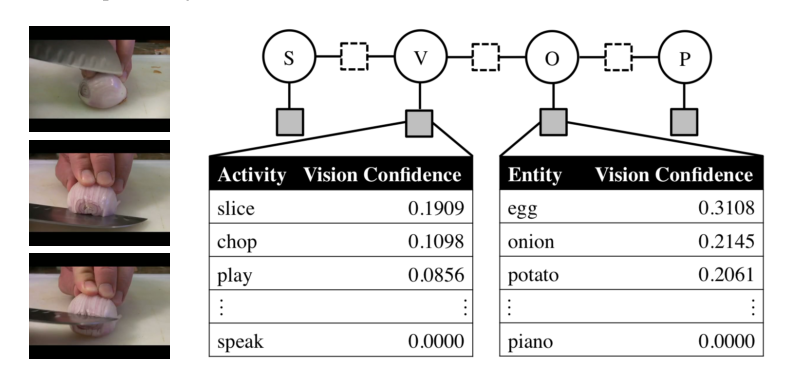
\includegraphics[width=120mm]{images/FactorGraph.png}
	\caption{مدل گراف فاکتور \label{text-mined-knowledge-model-2} \cite{Thomason2014}}
\end{figure}
در این روش، بعد از تعیین‌ توابع پتانسیل، با بهره‌گیری از تخمین بیشینه‌گر احتمال پسین 
\LTRfootnote{Maximum a posteriori}
(با استفاده از الگوریتم \LR{Max-product})، محتمل‌ترین مجموعه توامان از مقادیر را برای متغیر‌های نهان مد‌نظر به دست می‌آوریم. توابع پتانسیل تصویری و زبانی برای این مسئله، با در نظر گرفتن
$k \in \{S, V, O, P\}$
به صورت زیر تعریف شده‌اند:
\begin{equation}
 \phi_{k}(t) = C_k(t) \hspace{5mm}, \hspace{5mm} \phi_{k, l}(t, s)  = p(l = s | k = t) = \alpha p_0(l = s‌‌ | k = t) +‌(1 - \alpha) p_i (l = s | k = t)
\end{equation}
با توجه به این‌که مشاهدات تصویری مدل، به صورت یک توزیع احتمال در خواهند آمد پتانسیل تصویری هر عنصر (فعل، فاعل، مفعول و صحنه) $k$، میزان اطمینانی است که دسته‌بند برای عنصر $k$م به کلمه‌ی $t$م تخصیص می‌دهد.
در توابع پتانسیل زبانی، $k$ و $l$ دو عنصر پشت‌سر هم در دنباله‌ی $SVOP$ هستند که $s$ و $t$ مقادیر ممکن‌‌ برای آن دو عنصر را مشخص می‌کنند.

روش ایجاد جملات در این پژوهش تقریبا تفاوتی با پژوهش قبل ندارد و از همان روش قالب محور استفاده شده است.  تنها تفاوت در این گام، با توجه به افزوده شدن صحنه‌ به سه‌تایی فعل، فاعل و مفعول، بررسی لزوم نیاز جمله به  مفعول و صحنه‌ی تصویر است. در واقع با توجه به این‌که بعضی از افعال غیر متعدی هستند و یا ممکن است آوردن صحنه باعث تکرار مفاهیم شود، سه نوع متفاوت جمله از بهترین عناصر به دست آمده (\LR{SVO, SVP, SVOP}) ساخته می‌شوند و توسط مدل زبانی 
\cite{pauls2011faster}
امتیازدهی می‌شوند تا بهترین آنها به عنوان خروجی مدل انتخاب شود.

\subsection{ایجاد توصیف با استفاده از شبکه‌های ژرف بازگردنده}\label{rnns}
یکی از بزرگترین معایب روش‌های ذکر شده در جهت ایجاد توصیف برای ویدئو‌ها، استفاده از قالب‌های یکسان و به دست آوردن تعدادی قواعد معنایی ثابت (سه‌تایی یا چهار‌تایی‌های فعل، فاعل، مفعول و صحنه) برای ایجاد توصیف ویدئو به زبان‌طبیعی است. استفاده از این قالب‌های ثابت برای مجموعه کلمات بزرگتر مشکل می‌شود و همچنین جملات با قالب‌های از پیش تعیین شده و خشک، بسیار ساده‌تر از جملاتی خواهند بود که بتوانند به درستی ساختار پیچیده‌ی زبان‌طبیعی را ضبط و رعایت کنند.

در جهت رفع این مشکلات، نویسندگان‌ 
\cite{Donahue2015}
با توجه به موفقیت روش‌های یادگیری ژرف در فعالیت‌های توصیف تصاویر ساده، به استفاده از این روش‌‌ها روی آوردند. به طور خاص نویسندگان در این پژوهش  با استفاده از ترکیبی از شبکه‌های ژرف پیچشی و نوعی خاص از شبکه‌های ژرف بازگردنده به نام
\LR{LSTM}\LTRfootnote{Long Short‌ Term Memory}
مدلی را ارائه می‌کنند که با تغییرات کمی می‌تواند برای سه فعالیت بازشناسی کنش، توصیف تصویر و توصیف ویدئو استفاده شود. 

\subsubsection{شبکه‌های ژرف بازگردنده} \label{about-rnns}
شبکه‌های بازگردنده قابلیت یادگیری پویایی‌‌های زمانی پیچیده را با نگاشت دنباله‌ی ورودی به دنباله‌ای از حالات‌نهان با رابطه‌ی
$ h_t = g(W_{xh}x_t‌+‌W_{hh}h_t + b_h)$
و در ادامه نگاشت این حالات نهان به خروجی را  دارند. عملکرد این شبکه‌ها به این صورت است که هر ورودی تصویری $v_t$، از یک تابع غیر خطی استخراج ویژگی $\phi_v(v_t)$‌ که پارامتر آن $V$ است، عبور می‌کند تا در نهایت، یک بردار ویژگی با طول ثابت، $\phi_t \in \Re^d$، از تصویر ورودی به دست آید. بعد از این‌که ورودی تصویری به یک بردار ویژگی با طول ثابت تبدیل شد، نوبت به بخش دوم مدل، یعنی شبکه‌ی بازگردنده می‌رسد.
در کلی‌ترین حالت، یک مدل دنباله‌ای
 \LTRfootnote{Sequence Model}
 که پارامتر آن را ماتریس $W$ مشخص می‌کند، نگاشتی از ورودی‌های $x_t$ و حالت نهان زمان قبلی $h_{t-1}$، به یک خروجی در زمان فعلی $z_t$ و حالت نهان جدید $h_t$ به دست می‌دهد. سپس در قدم‌نهایی، برای به دست آوردن یک توزیع احتمالاتی مناسب روی کلمات خروجی محتمل در هر زمان، روی خروجی شبکه‌ی بازگردنده $z_t$ یک تابع 
 \LR{Softmax}
 اعمال می‌شود.
 \begin{equation*}
	 P(y_t=c) = \frac{\exp{(W_{zc}z_{t,c}‌+‌b_c)}}{\sum_{c' \in C} \exp{(W_{zc}z_{t,c}‌+‌b_c)}}
 \end{equation*}
 با توجه به رابطه‌ی بالا، حدس‌های نهایی مدل (نزدیک به $T$، تعداد فریم‌های ویدئو)، حدس‌هایی هستند که توسط یک شبکه‌ی بسیار ژرف زده می‌شوند. ماتریس وزن‌های $W$ نیز در این مدل، برای تمامی زمان‌ها مشترک است که این ویژگی، مدل را مجبور به یادگیری قواعدی کلی می‌کند که در میان زمان‌های متفاوت ثابت هستند که متقابلاً باعث کاهش بیش‌برارزش
 \LTRfootnote{Overfitting}
و کاهش پارامتر‌های شبکه خواهد شد. معماری کلی یک شبکه‌ی بازگردنده در سمت چپ شکل
 \ref{rnn-lstm}
  قابل مشاهده‌ است.

\begin{figure}[ht!]
	\centering
	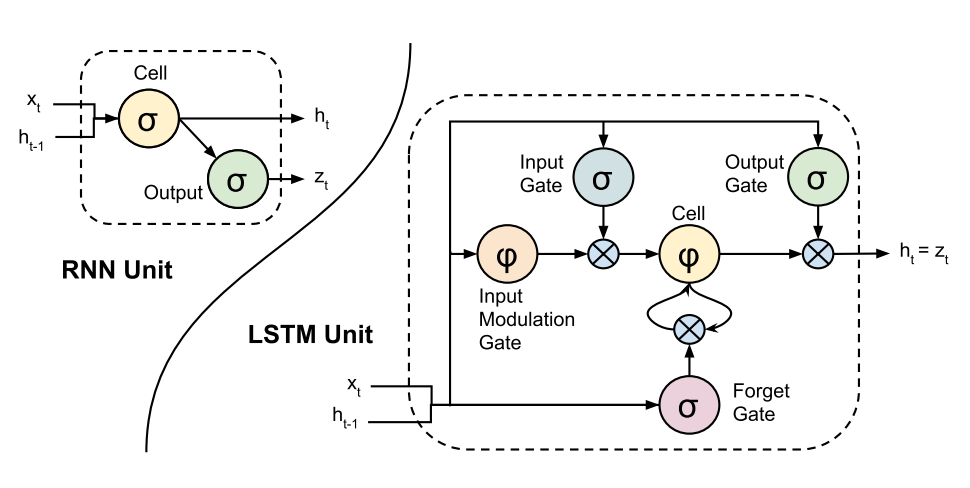
\includegraphics[width=120mm]{images/rnn-lstm.png}
	\caption{مدل LSTM و RNN \label{rnn-lstm}\cite{Donahue2015}}
\end{figure}

با این‌که شبکه‌های بازگردنده در زمینه‌هایی مانند بازشناسی گفتار و تولید متن موفق عمل کرده‌اند، آموزش‌‌دادن این دسته از مدل‌ها برای اینکه روی دنباله‌های طولانی پاسخ مناسبی دهند، کمی سخت است. در واقع در مراحل آموزش چنین مدل‌هایی با دو مشکل عمده مواجه می‌شویم، ناپدید شدن 
\LTRfootnote{Vanishing Gradients}
و یا بسیار بزرگ شدن 
\LTRfootnote{Exploding Gradients}
مقادیر بردار گرادیان است، که به دلیل گذرانده‌شدن گرادیان‌ها از تعداد لایه‌های زیاد شبکه در زمان یادگیری است. برای حل این مشکل، مدلی بازگردنده به نام 
\LR{LSTM}
در پژوهش 
\cite{hochreiter1997long}
 ارائه شده است. \LR{LSTM}ها با معماری خاص خود، به شبکه اجازه می‌دهند تا در فاز آموزش، شبکه یاد‌بگیرد که در چه زمانی حالت‌های نهان قبلی را فراموش کند و در چه زمانی حالت‌نهان فعلی را با اطلاعات جدید به روز‌رسانی کند. معماری یک سلول
\LR{LSTM}
در قسمت راست شکل  \ref{rnn-lstm} قابل رویت است. با نمایش دادن تابع سیگموید با $\sigma$ و تابع تانژانت هایپربولیک با $\phi$ روابط به روز‌رسانی سلول‌ها در \LR{LSTM} به صورت زیر خواهد بود.
\begin{align*}
	& i_t = \sigma(W_{xi}x_t + W_{hi}h_{t-1}‌ +‌ b_i )& & f_t = \sigma(W_{xf}x_t +‌W_{hf}h_{t-1}‌‌+b_f) &&‌ o_t = \sigma(W_{xo}x_t‌+‌w_{ho}h_{t-1} + b_o) \\
	& g_t = \phi(W_{xc}x_t + W_{hc}h_{t-1} + b_c) & & c_t = f_t  * c_{t-1}‌+ i_t * g_t  && h_t = o_t  * \phi(c_t)
\end{align*}

\subsubsection{روش ارائه شده}
معماری پایه‌ی روش ارائه شده در شکل \ref{lrcn-1} قابل مشاهده است. نویسندگان در این مقاله از یک شبکه‌ی عصبی پیچشی برای استخراج ویژگی از تصاویر استفاده کرده‌اند. خروجی آخرین لایه‌های کاملا متصل شبکه‌ی پیچشی (لایه‌های $fc_7$ و $fc_6$)، به عنوان ورودی $d$ بعدی $x_t$ برای شبکه‌ی بازگردنده در نظر گرفته می‌شوند.
\begin{figure}[ht!]
	\centering
	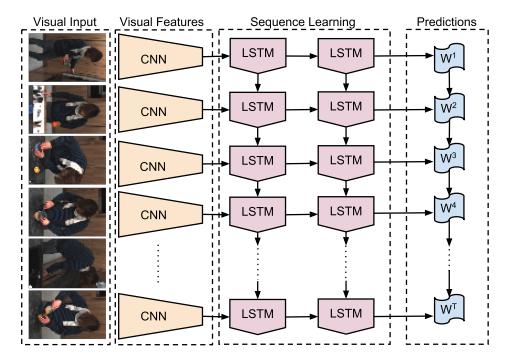
\includegraphics[width=120mm]{images/lrcn-1.png}
	\caption{مدل LRCN \label{lrcn-1}\cite{Donahue2015}}
\end{figure}

نویسندگان این پژوهش، با ارائه‌ی تعریفی از معماری پایه‌ی شبکه، اقدام به تعریف سه زیر مسئله که با معماری ارائه شده قابل حل است می‌کنند.  مسائل تعریف شده شامل مسائل با ورودی دنباله‌ای و خروجی ثابت (تشخیص عمل در ویدئو)، ورودی ثابت و خروجی دنباله‌ای (توصیف تصویر) و در نهایت مسائل با ورودی و خروجی دنباله‌ای (توصیف ویدئو) هستند.

در حالت اول، از یک روش درهم‌آمیزی دیرهنگام برای به دست آوردن پاسخ نهایی شبکه از پاسخ‌های مبتنی بر زمان شبکه استفاده می‌شود.  در حالت دوم که ورودی ثابت است و خروجی دنباله‌ای شکل، نویسندگان با تکرار کردن ورودی ثابت در هر زمان $t$ مسئله را به حالت بعدی یعنی ورودی و خروجی دنباله‌ای تبدیل می‌کنند. در این حالت از یک مدل انکودر-دیکودر 
\LTRfootnote{Encoder-Decoder}
استفاده می‌شود. در این روش یک دنباله توسط انکودر به یک بردار با طول ثابت نگاشت می‌شود. سپس یک مدل دنباله‌ای دیگر که دیکودر نامیده می‌شود، بردار خروجی انکودر را به دنباله‌ای با طول متغیر تبدیل می‌کند. در واقع در این معماری، سیستم دارای $T+T'$ گام زمانی است که در $T$ گام ابتدای پردازش روی ورودی انجام می‌شود و از خروجی چشم‌پوشی می‌شود. سپس در $T'$ گام بعدی، خروجی از مدل دیکودر گرفته می‌شود.
با در نظر گرفتن معماری توضیح داده‌شده، پارامتر‌های $V$ و $W$ که به ترتیب مربوط به مدل تصویری و دنباله‌ای هستند، می‌توانند با بهینه‌سازی درست‌نمایی برچسب‌های خروجی $y_t$ مشروط به ورودی و حالت‌نهان تا آن زمان، محاسبه شوند.
\begin{align*}
L(V, W) = -\log P_{V,W}(y_t‌|‌x_{1:t}, y_{1:t-1})
\end{align*}
در این پژوهش برای ایجاد توصیف برای ویدئو از یک
\LR{CRF} \LTRfootnote{Conditional‌ Random Field}
استفاده شده است. دلیل این امر، نبود مجموعه‌دادگان مناسب و کافی برای آموزش مدلی بر مبنای شبکه‌های عصبی پیچشی است. \LR{CRF} استفاده شده در این بخش از پژوهش با دریافت ویژگی‌های دست‌ساز از ویدئو‌ی ورودی، سه‌تایی فعل، فاعل و مفعول را تولید می‌کند و به عنوان ورودی به انکودر وارد می‌کند.  در نهایت سه معماری متفاوت (شکل \ref{lrcn-captioning}) برای اتصال عناصر پیشنهاد شده‌ است که با توجه به بررسی انجام شده مدل \LR{C} بهترین دقت را در معیار \LR{BLEU-4} دارا است. در این معماری انکودر حذف شده و بردار احتمال مرتبط با کلمات انتخاب شده توسط \LR{CRF} در هر گام‌زمانی به عنوان ورودی دیکودر تکرار می‌شوند. 
\begin{figure}[ht!]
	\centering
	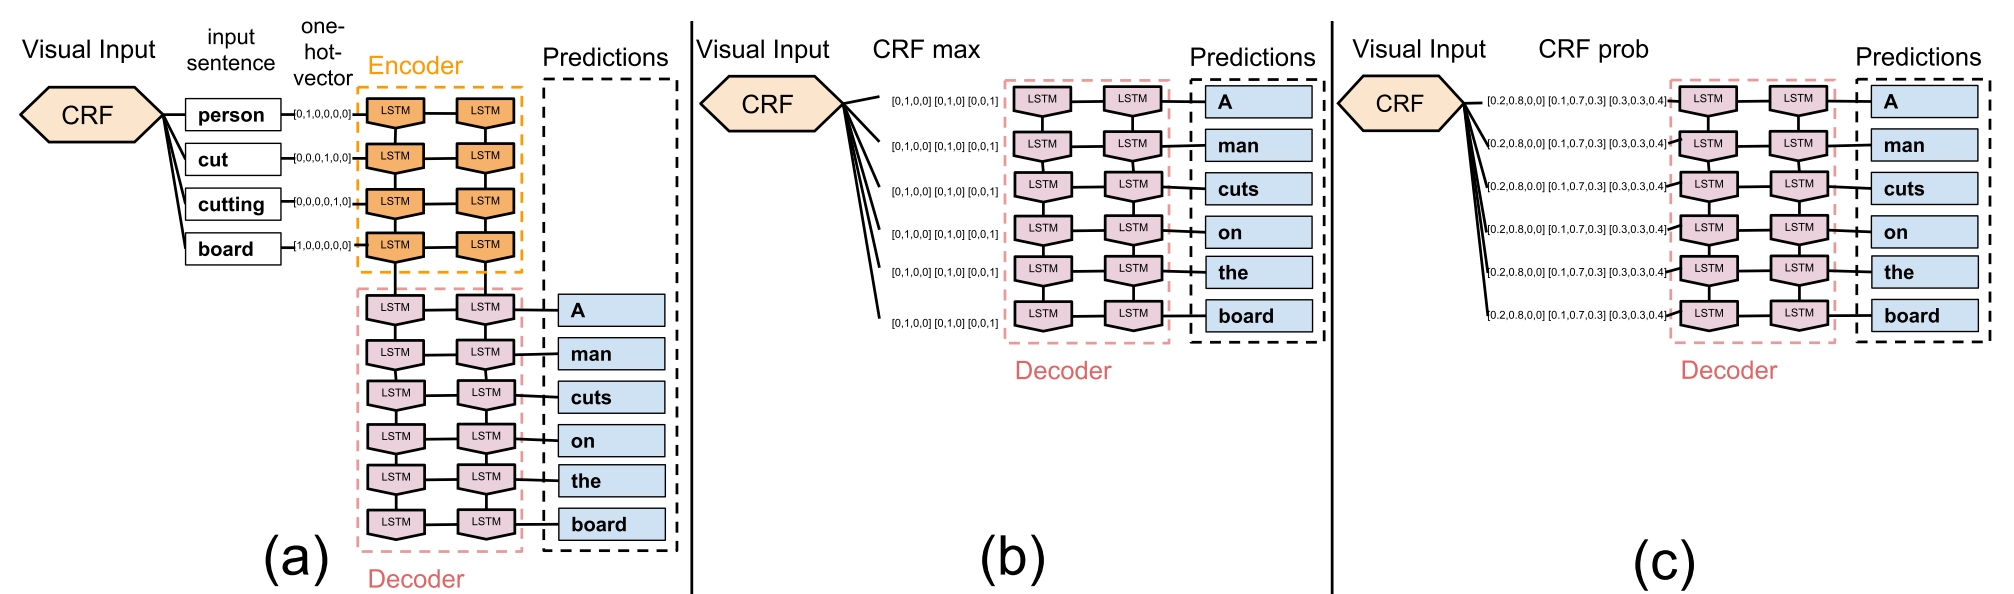
\includegraphics[width=170mm]{images/lrcn-captioning.png}
	\caption{نمونه‌های معماری پایه برای توصیف ویدئو\label{lrcn-captioning}\cite{Donahue2015}}
\end{figure}


پژوهش
 \cite{Venugopalan2015}
  که بعد از این پژوهش انجام شد، دو مشکل اساسی آن را در زمینه‌ی توصیف ویدئو برطرف می‌کند. در واقع در این پژوهش با استفاده از شبکه‌ی پیچشی به جای 
\LR{CRF}
باعث می‌شود مدل قابلیت آموزش به صورت انتها‌به‌انتها
\LTRfootnote{End-to-End}
را به دست آورد و همچنین نیاز به تعیین ویژگی‌ها و نقش‌های معنایی به صورت دستی (که برای مجموعه‌لغات بزرگ بسیار مشکل است) از بین رود. در این مدل به آموزش مدلی پرداخته‌ شده‌است که با توجه به ویژگی‌های تصویری $V$ و کلمات قبلی تولید شده توسط مدل،
 $S_1, \cdots , S_{t-1}$
 ، احتمال درست‌نمایی جمله $S$ را بیشینه کند.
 \begin{align}
	 \theta^* = \argmax_\theta \sum_{V,S}\log p(S|V; \theta)  \rightarrow \log p(S|V) = \sum_{t=0}^N \log p(S_{w_t}|V, S_{w_1}, \cdots, S_{w_{t-1}})
 \end{align}‌
 در این مدل از یک‌ شبکه‌ی پیچشی که در کتابخانه‌ی 
 \LR{Caffe} \cite{jia2014caffe}
 موجود است (شبکه‌ی عصبی 
 \LR{AlexNet} \cite{krizhevsky2012imagenet}
  ) استفاده شده است که روی ۱.۲ میلیون تصویر از مجموعه‌داده‌ی 
  \LR{ILSVRC-2012}\cite{russakovsky2015imagenet} 
پیش‌آموزش داده‌‌ شده است. از هر ۱۰ فریم ویدئو یک فریم نمونه‌گیری شده است و از خروجی لایه‌ی آخر کاملا متصل شبکه پیچشی (
\LR{$fc_7$}
) به عنوان بردار ۴۰۹۶ بعدی نمایش‌گر ویدئو استفاده شده است. ورودی انکودر برداری است که از کنار هم گذاشتن بردار ویژگی‌های ویدئو و همچنین بردار ویژگی کلمه‌ی ایجاد شده‌ی قبلی به دست می‌آید. ورودی دیکودر نیز خروجی انکودر در هر گام زمانی است. در نهایت با اعمال تابع \LR{Softmax} روی خروجی دیکودر، کلمه با بالاترین احتمال را به عنوان خروجی انتخاب می‌کنیم. با اعمال تغییرات ذکر شده، بهبود ۲درصد در معیار \LR{BLEU-4} نسبت به پژوهش قبلی مشاهده می‌شود.
 \subsection{بهبود توصیف متنی بر شبکه‌های بازگردنده با استفاده از دانش متن‌کاوی شده}\label{rrns-and-text-mined-knowledge}
 در ادامه‌ی پژوهش قبلی، در پژوهش 
\cite{Venugopalan2016}
نویسندگان مدل زبانی ارائه شده را به شکلی تغییر می‌دهند تا از دانش داده‌کاوی شده از متون موجود در اینترنت نیز بهره ببرد. برای مخلوط کردن دانش موجود از متون با مدل‌زبانی ارائه شده در پژوهش قبلی، از سه روش ادغام سریع
\LTRfootnote{Early Fusion}
، ادغام دیر‌هنگام
\LTRfootnote{Late Fusion}
 و ادغام ژرف 
 \LTRfootnote{Deep‌‌ Fusion}
 استفاده شده‌است. در روش ادغام سریع، بخش‌هایی از شبکه که زبان‌طبیعی را مدل می‌کنند، روی متون موجود، پیش‌آموزش داده می‌شوند و در نهایت روی متون مرتبط با مجموعه‌ی داده، تنظیم دقیق
 \LTRfootnote{Finetune}
 می‌شوند. دو روش دیگر از یک \LR{LSTM} مجزا، که روی متون موجود اینترنت، از پیش‌ آموزش داده شده‌اند استفاده می‌کنند. همچنین در این پژوهش به جای نمایش کلمات به صورت \LR{One-Hot} (نحوه‌ای از نمایش که هر کلمه به صورت برداری به طول تمامی مجموعه لغات نمایش داده می‌شود که تنها در نمایه‌ی مرتبط با کلمه‌ی فعلی مقدار آن برابر با یک و در دیگر نقاط مقدار آن صفر است)، از روش‌های بازنمایش آماری کلمات از پیش آموزش‌دیده شده، استفاده می‌شود. مزیت استفاده از این دست نمایش‌ها برای کلمات، کاهش قابل توجه ابعاد داده‌ها‌ی زبانی و همچنین استفاده از مفاهیم موجود در کلمات است.
 
 \subsubsection{ادغام دیر‌هنگام}
استفاده‌ی روش ادغام دیرهنگام از شبکه‌های پیش‌آموزش دیده، مشابه استفاده‌ی روش‌های ترجمه‌ی ماشینی زبان، در دیکودر است. در هر مرحله از ایجاد جمله، مدل توصیف ویدئو یک توزیع روی کلمات ایجاد می‌کند. خروجی نهایی با در نظر‌گرفتن میانگین وزن‌دار مجموع امتیازات داده‌شده توسط مدل‌زبانی و مدل موجود توصیف ویدئو ایجاد می‌شود. به طور دقیق‌تر، با در نظر گرفتن $y_t$ به عنوان خروجی مدل در زمان $t$، 
 $P_{VM}$
 و
 $P_{LM}$
 به عنوان توزیع‌هایی که به ترتیب مدل‌های توصیف ویدئو و زبان تولید می‌کنند، برای تمامی لغات خروجی می‌توان تابع امتیاز زیر را در نظر گرفت:
\begin{align*}
	p(y_t=y') = \alpha P_{VM}(y_t=y') +‌ (1-\alpha) P_{LM}(y_t=y')
\end{align*}

\subsubsection{ادغام ژرف}
در روش ادغام ژرف، مدل‌زبانی جداگانه به صورت ژرف‌تری با مدل ترکیب می‌شود (برخلاف ادغام دیر‌هنگام که تنها در انتهای مدل از مدل‌زبانی دارای دانش استفاده شده بود). نحوه‌ی انجام این‌کار بدین صورت است که حالت‌نهان مدل زبانی مجزا
 \LR{LSTM $(h_t^{LM})$}
 در کنار حالت‌نهان مدل توصیف ویدئو موجود 
 \LR{$h_t^{VM}$}
 قرار داده می‌شود و از بردار حاصله‌ی جدید برای پیش‌بینی کلمه‌ی فعلی استفاده می‌شود. احتمال انتخاب یک کلمه‌ی خاص در زمان $t$ در این مدل متناسب با رابطه‌ی زیر است:
 \begin{equation*}
	 p(y_t|y_{<t}, v) \propto \exp(Wf(h_t^{VM}, h_t^{LM}) + b)
 \end{equation*}
 در این رابطه، $b$ و $v$ به ترتیب بایاس و بردار ویژگی‌های تصویر را نمایش می‌دهند. برای جلوگیری از بیش‌برازش مدل به وزن‌های پیش‌آموزش داده‌ شده‌ی مدل زبانی، وزن‌های این مدل در مرحله‌ی آموزش ثابت نگه‌داشته می‌شوند و تنها وزن‌های شبکه‌ی توصیف ویدئو موجود به روز‌رسانی می‌شوند تا از وزن‌های مدل‌زبانی نیز در به دست آمدن وزن‌های نهایی استفاده شده باشد.
 \subsubsection{نمایش توزیعی کلمات}
 شبکه‌ی توصیف ویدئو موجود، مانند بسیاری از مدل‌های توصیف ویدئو و تصویر دیگر، از نمایش \LR{One-Hot} برای کلمات استفاده می‌کند. در این حالت در زمان آموزش، بخش مرتبط با زبان شبکه، با استفاده از داده‌های آموزش، یک نمایش با ابعاد کمتر (۵۰۰ بعدی) از کلمات را یاد می‌گیرد. اما این یادگیری از داده‌هایی محدود و دارای نوفه موجود در مجموعه‌دادگان رخ می‌دهد که بهینه نیست.  روش‌های زیادی هستند که برای حل این مشکل، یک مدل همه‌منظوره روی متون بسیار زیاد آموزش می‌دهند تا بتوان از آنها در مدل‌های دیگر استفاده کرد. در این پژوهش از نمایش بردار‌های 
 \LR{GloVe} \cite{pennington2014glove}
 استفاده شده است که کلمات را در قالب یک بردار ۳۰۰ بعدی نمایش می‌دهد. در نهایت هم با توجه به غیر محدب بودن تابع هزینه‌ی شبکه، از میانگین خروجی چندین نمونه‌ی متفاوت  
 \LTRfootnote{Ensemble}
 از مدل، به عنوان خروجی نهایی استفاده شده است.
 اعمال تغییرات آورده‌ شده در این پژوهش، منجر به افزایش دقت ۵ درصدی در معیار
  \LR{BLEU-4}
   و ۲.۴ درصدی در معیار
    \LR{Meteor}
 در مجموعه داده‌گان یوتیوب شده است.
 \subsection{ایجاد توصیف با استفاده از شبکه‌های ژرف بازگردنده چند سطحی}\label{hierarchical-rnns}
از نقاط ضعف روش‌های پیشین می‌توان به دو مورد اصلی اشاره کرد. مورد اول این‌که این روش‌ها عموما برای بهبود جملات روی مدل زبانی شبکه تمرکز می‌کردند و به ویژگی‌های تصویری استخراج شده توسط شبکه‌ی پیچشی بسنده می‌کردند. مورد دوم این‌که در این روش‌ها، تنها یک جمله به عنوان خروجی مدل ایجاد می‌شد که گاهاً جهت توضیح یک ویدئو‌ی پرمحتوا، به هیچ عنوان کافی نیست. در پژوهش 
\cite{Yu2016}
نویسندگان با ارائه‌ی یک معماری پیچیده‌تر، سعی در رفع مشکلات اشاره شده دارند.

در این پژوهش، یک شبکه‌ی عصبی ژرف بازگردنده چند‌سطحی برای توصیف ویدئو‌های طولانی با چندین پاراگراف ارائه شده است. با توجه به اینکه در هر پاراگراف، جملات باید مرتبط با یکدیگر ایجاد شوند، شبکه‌ی چند‌سطحی از دو ایجاد کننده
\LTRfootnote{Generator}
، یک ایجاد‌کننده‌ی جمله و یک ایجاد‌کننده‌ی پاراگراف، تشکیل می‌شود. در سطح پایین، وظیفه‌ی ایجادکننده‌ی جمله تولید جملاتی است که یک بازه‌ی زمانی کوتاه و مشخص در ویدئو را توصیف می‌کنند.  در این پژوهش از مکانیزم توجه 
\LTRfootnote{Attention}
در هر دو حوزه‌ی زمان \LTRfootnote{Temporal‌‌‌ Attention}و مکان \LTRfootnote{Spatial Attention}، جهت انتخاب دقیق‌تر المان‌های تصویری مرتبط با جمله‌ی در حال تولید، استفاده شده است. در سطح بالاتر، نمایشی از جملات ایجاد شده را به عنوان ورودی دریافت می‌کند و وضعیت پاراگراف با به عنوان خروجی ایجاد می‌کند، این خروجی (وضعیت پاراگراف) به عنوان حالت اولیه به شبکه‌ی ایجاد‌کننده‌ی جملات داده می‌شود. هرکدام از این شبکه‌ها، یک شبکه‌ی بازگردنده خاص به نام
 \LR{GRU} \cite{chung2014empirical}
هستند که مدل ساده‌ شده‌ی \LR{LSTM}ها هستند که در قسمت‌ قبل معرفی شدند. معماری کلی شبکه‌ی نهایی در شکل \ref{hrnn} قابل مشاهده است.

\begin{figure}[ht!]
	\centering
	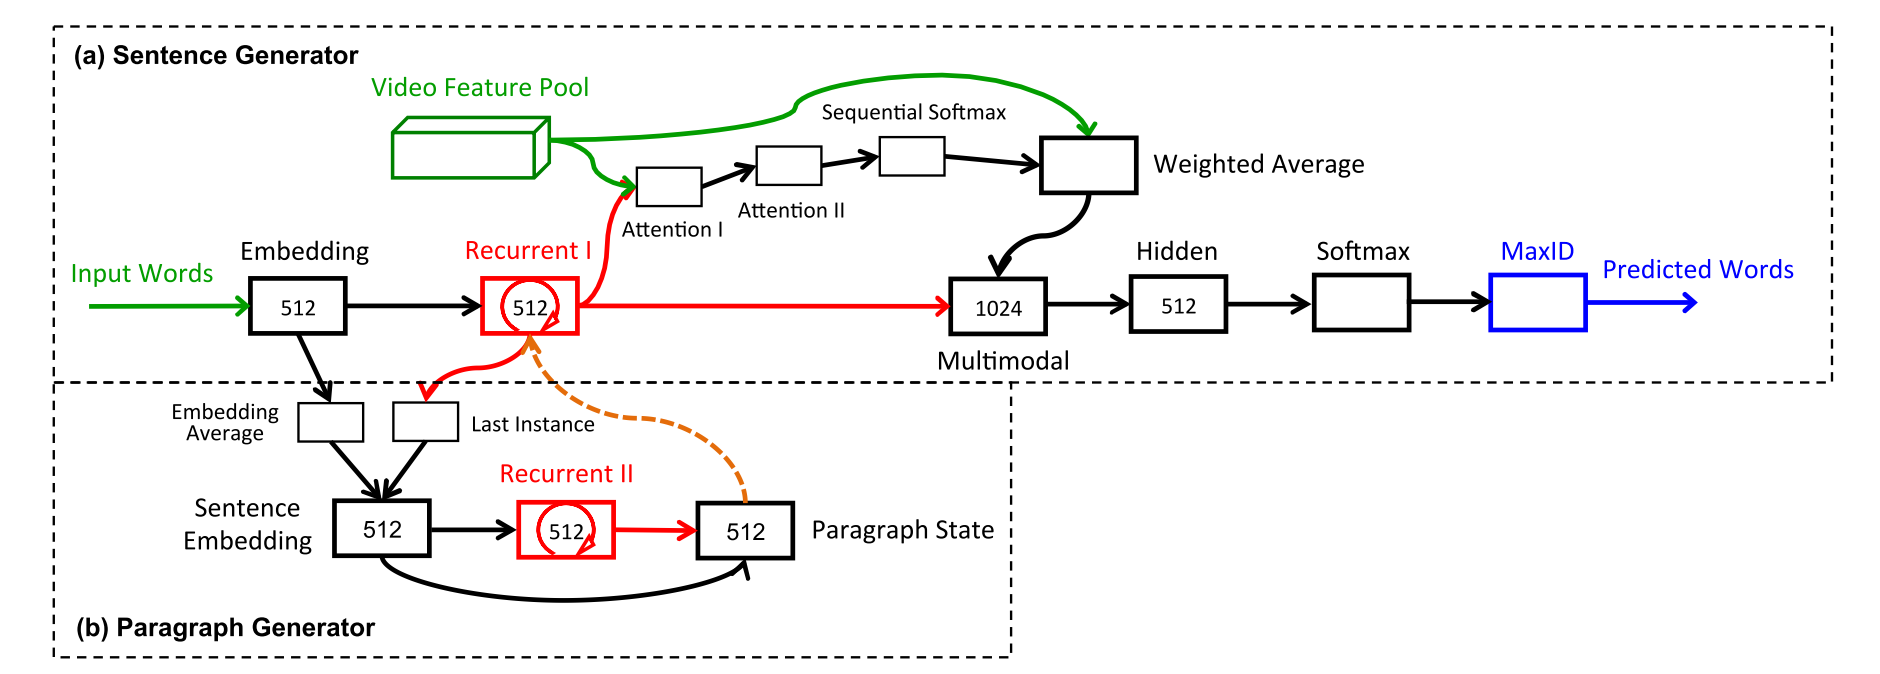
\includegraphics[width=170mm]{images/hrnn.png}
	\caption{شبکه‌ی بازگردنده چند سطحی برای توصیف ویدئو\label{hrnn}}
\end{figure}

\subsubsection{ایجاد‌کننده‌ی جمله}
این شبکه در هر گام زمانی با ورود یک بردار \LR{One-Hot} از کلمه‌، با استفاده از یک جدول تعبیه
\LTRfootnote{Embedding}
، بردار ورودی را به یک بردار فشرده‌تر (۵۱۲ بعد) تبدیل می‌کند. سپس مانند روش‌های پیشین، بردار فشرده‌ی به دست آمده وارد لایه‌ی بازگردنده ۱، شبکه‌ی انکودر می‌شود. تفاوت این شبکه با شبکه‌ی مدل‌های قبلی در استفاده از \LR{GRU} به جای \LR{LSTM} است. همچنین به عنوان تابع فعال‌سازی از تابع \LR{ReLu} \LTRfootnote{Rectified Linear Unit} به جای تابع سیگموید استفاده شده است. خروجی شبکه‌ی ۱، به لایه‌های توجه \LTRfootnote{Attention‌ Layers}  داده می‌شوند تا ضرایب توجه برای ویژگی‌های تصویر به دست آیند. ضرایب توجه، با در نظر گرفتن یک توزیع احتمال روی ویژگی‌های هر فریم در هر زمان به دست می‌آید. اگر ویژگی‌های موجود در ویدئو رو با 
$v_1, \cdots, v_{KM}$
نشان‌دهیم که در آن $M$ طول ویدئو و $K$ تعداد وصله‌ها \LTRfootnote{Patch} روی هر فریم است. هدف، به دست آوردن مجموعه‌ای از ضرایب 
$\beta^t_1, \cdots, \beta^t_{KM}$
در هر زمان، به طوری که 
$\sum_{m=1}^{KM} \beta_i^t = 1$
است. برای این‌کار ابتدا امتیاز توجه برای هر فریم $m$ محاسبه‌ می‌شود.
\begin{equation*}
	q_m^t = W^T \phi(W_qv_m +‌U_qh^{t-1} + b_q)
\end{equation*}
که در آن، $\phi$ تابع $stanh$ در نظر گرفته شده است. سپس با گرفتن \LR{Softmax} از امتیاز‌های توجه به دست آمده، امتیاز توجه برای هر ویژگی به دست می‌آید:
\begin{equation*}
		\beta^t_m = \frac{\exp(q_m^t)}{\sum_{m'=1}^{KM} \exp(q^t_{m'})}
\end{equation*}
در نهایت بردار ویژگی‌نهایی در لایه‌ی میانگین وزن‌دار، با ضرب ضرایب به دست آمده از لایه‌ی توجه در بردار ویژگی‌های تصویر به دست می‌آید: 
\LR{$u^t = \sum_{m=1}^{KM}$}.
در ادامه خروجی لایه‌ی میانگین وزن‌دار ویژگی‌های تصویر (۱۰۲۴ بعدی)، به همراه خروجی لایه‌ی بازگردنده ۱، وارد لایه‌ی چند‌حالته می‌شوند. در این لایه، عناصر تصویر و متن بایکدیگر مخلوط می‌شوند. برای حالتی که ویژگی‌های تصویری دو کاناله باشند ($u_a$ و $u_o$)، خروجی این لایه (\LR{$m^t$}) برابر با
$\phi(W_{m,o}u_o^t +‌W_{m,a}u_a^t +‌U_mh^t+b_m)$
 است.
\subsubsection{ایجاد‌کننده‌ی پاراگراف}
ایجاد‌کننده‌ی جمله در مرحله‌ی قبل، عملیات مرتبط با یک‌جمله را انجام می‌دهد. حالت اولیه‌ی لایه‌ی بازگردنده ۱ برای اولین جمله برابر با صفر در نظر گرفته می‌شود، اما بعد از ایجاد اولین جمله، حالت اولیه این لایه، با توجه به معنی مفهومی جملات قبل، توسط ایجاد‌کننده‌ی پاراگراف تنظیم می‌شود. در مراحل ایجاد یک جمله، میانگین تعبیه‌شده‌‌های تمامی کلمات جمله توسط لایه‌ی میانگین تعبیه 
\LTRfootnote{Embedding Average Layer}
نگه‌داشته می‌شود که در کنار آخرین وضعیت لایه‌ی بازگردنده ۱ به عنوان حالت جمله، به عنوان ورودی لایه‌ی تعیبه‌ی جمله 
\LTRfootnote{Sentence Embedding} 
در نظر گرفته می‌شوند. خروجی این لایه‌، لایه‌ی بازگردنده ۲ است. این لایه زمانی لایه‌ی بعدی، که حالت پاراگراف است، را به روز‌رسانی می‌کند که نشان‌گر انتهای جمله 
\LTRfootnote{End Of Sentence,‌ EOS}
توسط ایجاد کنند‌ه‌ی جمله تولید شده باشد.
\subsubsection{آموزش}
با در نظر گرفتن $s_{1:t-1}$ به عنوان جملات قبلی موجود در پاراگراف و $w_{1:t-1}^n$ به عنوان کلمات قبلی موجود در جمله‌ی $n$م، تابع درست‌نمایی ایجاد یک کلمه به صورت
\LR{$p(w_t^n|s_{1:n-1}, w_{1:t-1}^n, V)$}
خواهد بود. با توجه به این تعریف، تابع هزینه ایجاد یک پاراگراف برابر است با:
\begin{align*}
	L(s_{1:N}|V) = - \frac{\sum_{n=1}^{N}\sum_{t=1}^{T_n}\log P(w_t^n|s_{1:n-1}, w_{1:t-1}^n, V) }{\sum_{n=1}^{N}T_n}
\end{align*}
در این رابطه، $T_n$ و $N$ به ترتیب تعداد کلمات موجود در جلمه‌ی $n$م و تعداد جملات موجود در پاراگراف است. با در نظر گرفتن پاراگراف‌های متعدد برای هر داده‌ی آموزش، تابع هزینه‌ی نهایی به صورت زیر به دست می‌آید:
\begin{align*}
	L = -\frac{\sum_{y=1}^{Y}\sum_{n=1}^{N_y}\sum_{t=1}^{T_n^y} \log P(w_t^{n, y}|s_{1:n-1}^y, w_{1:t-1}^{n, y}, V_y) }{{\sum_{y=1}^{Y}\sum_{n=1}^{N_y}T_n^y}}
\end{align*}
معماری ارائه شده در این پژوهش منجر به بهبود دقت در معیارهای
 $BLEU$
به میزان ۵ درصد و در معیار $METEOR$ به میزان ۲ درصد می‌شود.
\subsection{سایر روش‌ها}\label{other}
روش‌های متعدد دیگری برای توصیف ویدئو ارائه شده‌اند که فصل مشترک عموم این روش‌ها، استفاده از شبکه‌های پیچشی برای استخراج ویژگی و استفاده از شبکه‌های بازگردنده برای مدل‌کردن زبان طبیعی و ایجاد جملات است. در 
\cite{Pan2015}
نویسندگان، برخلاف پژوهش ارائه شده در 
\cite{Donahue2015}
از یک معماری انکودر-دیکودر ساده برای مدل زبانی استفاده می‌کنند، اما با تغییر مدل مربوط به ویژگی‌های تصویری و افزودن مکانیزم توجه و تعریف نوعی خاص از شبکه‌های بازگردنده، به دقتی بهتر از پژوهش ارائه شده در بخش
\ref{text-mined-knowledge}
و تقریبا معادل با دقت پژوهش ارائه شده در بخش \ref{rnns} می‌رسند.

در پژوهش 
\cite{Hendricks2016}
نویسندگان، با استفاده از دانش موجود در مدل زبانی پیش‌آموزش داده‌شده روی متون خارج از دامنه، راه‌حلی برای توصیف اشيا جدید که در زمان آزمون دیده‌نشده‌اند ارائه می‌کنند. در این پژوهش با استفاده از ماژول‌های موجود، یک لایه‌ی جدید چند‌حالته برای ترکیب دانش زبان‌طبیعی موجود و ویژگی‌های تصویری و انتقال دانش 
\LTRfootnote{Transfer Learning}
 ارائه شده است. در این مدل، دو شبکه‌ی مجزا روی مجموعه‌دادگان مجزا آموزش داده می‌شوند. برای مدل‌کردن زبان از یک شبکه‌ی بازگردنده و برای استخراج ویژگی‌های تصویری از یک شبکه‌ی پیچشی استفاده می‌شود. هر دو شبکه‌ی ذکر شده روی مجموعه‌دادگان جدا، شامل اشيا‌یی که در مجموعه‌دادگان اصلی حضور ندارند، پیش‌آموزش داده شده‌اند. در نهایت تمامی شبکه روی مجموعه‌ی دادگان اصلی آموزش داده می‌شود. در این شبکه وظیفه‌ی لایه‌ی چندحالته مخلوط کردن ویژگی‌های تصویری و زبانی و به دست آوردن یک‌ باز‌نمایش مناسب از اشیایی که در تصویر هستند و در مجموعه‌ی دادگان حضور ندارند است. برای این‌کار یک تابع هزینه‌ برای این لایه در نظر گرفته شده است که پیش‌بینی مدل‌های مجزا و مدل توصیف تصویر اصلی مدل را با یکدیگر مخلوط می‌کند.




